\section{Results}
\label{sec:results}

\subsection{Model-Level Scientific Collaboration}
\label{sec:model-results}
% Model rows and provider layout: Overleaf commit 3aa9990.
% Haiku: preserve local results updated 2026-10-06 (behavioral means and CIs supplied by collaborator, 2026-10-07).
\begin{table}[!htbp]
\centering
\begingroup
\footnotesize
\setstretch{1.0}
\setlength{\tabcolsep}{3pt}
\renewcommand{\arraystretch}{1.2}

\begin{tabular*}{\linewidth}{@{\extracolsep{\fill}}lcccc@{}}
\toprule
Actor model
& \shortstack{Persona-off\\performance}
& \shortstack{Mean Persona\\Performance}
& \shortstack{Fact\\recovery (\%)}
& \shortstack{Self-\\repetition (\%)} \\
\midrule

% =========================
% Anthropic Claude
% =========================
\multicolumn{5}{l}{
\raisebox{-0.15em}{

\includegraphics[height=1.05em]{figures/logos/anthropic.pdf}
}
\hspace{0.3em}
\textit{Anthropic Claude}
} \\[-1pt]

Claude Opus 5.5
& \shortstack{49.48\\{\scriptsize [45.02, 54.14]}}
& \shortstack{50.55\\{\scriptsize [48.15, 53.06]}}
& \shortstack{98.95\\{\scriptsize [97.83, 99.86]}}
& \shortstack{16.23\\{\scriptsize [14.79, 17.72]}}
\\

Claude Haiku 4.5
& \shortstack{21.97\\{\scriptsize [16.25, 27.71]}}
& \shortstack{19.72\\{\scriptsize [15.19, 24.14]}}
& \shortstack{67.95\\{\scriptsize [61.77, 74.37]}}
& \shortstack{21.43\\{\scriptsize [17.23, 24.53]}}
\\

\addlinespace[3pt]

% =========================
% Google Gemini
% =========================
\multicolumn{5}{l}{
\raisebox{-0.15em}{

\includegraphics[height=1.05em]{figures/logos/gemini.pdf}
}
\hspace{0.3em}
\textit{Google Gemini}
} \\[-1pt]

Gemini 3.7 Flash
& \shortstack{48.21\\{\scriptsize [42.73, 53.77]}}
& \shortstack{48.17\\{\scriptsize [45.56, 50.83]}}
& \shortstack{75.24\\{\scriptsize [67.27, 82.79]}}
& \shortstack{13.08\\{\scriptsize [11.05, 15.13]}}
\\

Gemini 3 Flash
& \shortstack{33.07\\{\scriptsize [28.55, 37.91]}}
& \shortstack{31.98\\{\scriptsize [29.46, 34.42]}}
& \shortstack{90.01\\{\scriptsize [85.65, 93.85]}}
& \shortstack{13.43\\{\scriptsize [11.72, 15.23]}}
\\

\addlinespace[3pt]

% =========================
% OpenAI GPT
% =========================
\multicolumn{5}{l}{
\raisebox{-0.15em}{

\includegraphics[height=1.05em]{figures/logos/openai.pdf}
}
\hspace{0.3em}
\textit{OpenAI GPT}
} \\[-1pt]

GPT-6 Astra
& \shortstack{47.54\\{\scriptsize [39.11, 55.46]}}
& \shortstack{48.82\\{\scriptsize [40.46, 56.67]}}
& \shortstack{88.86\\{\scriptsize [76.96, 97.68]}}
& \shortstack{12.69\\{\scriptsize [11.65, 13.73]}}
\\

GPT-5 mini
& \shortstack{26.37\\{\scriptsize [22.19, 30.94]}}
& \shortstack{31.63\\{\scriptsize [28.32, 35.10]}}
& \shortstack{68.42\\{\scriptsize [60.71, 75.99]}}
& \shortstack{10.52\\{\scriptsize [8.78, 12.33]}}
\\

GPT-5 nano
& \shortstack{14.56\\{\scriptsize [10.41, 18.69]}}
& \shortstack{15.55\\{\scriptsize [13.29, 17.83]}}
& \shortstack{63.26\\{\scriptsize [55.83, 70.76]}}
& \shortstack{15.99\\{\scriptsize [13.70, 18.44]}}
\\

\bottomrule
\end{tabular*}

\endgroup

\caption{
\textbf{Model-level scientific collaboration scorecard.}
Means with 95\% confidence intervals.
Haiku fact recovery and self-repetition, including their 95\% confidence intervals, are collaborator-reported; the interval computation method has not been independently verified.
Performance uses scores normalized to 0--100; persona means weight the four profiles equally.
GPT-6 Astra uses low reasoning effort.
Each actor also serves as its researcher simulator; model-based judging uses GPT-6 Astra.
}

\label{tab:model-scorecard}
\end{table}


Across the seven reported model configurations, the difference between
mean persona performance and persona-off performance varied in both
direction and magnitude (\tabref{tab:model-scorecard}). GPT-5 mini showed
the largest observed increase, from 26.37 under persona off to 31.63
across the four personas, a difference of 5.26 points. Gemini 3.7 Flash
had nearly identical means under the two settings (48.21 and 48.17,
respectively). Evaluating multiple researcher settings therefore reveals
variation in scientific performance that a single persona-off score
cannot capture.

The model configurations also showed contrasting strengths in task
performance and interaction behavior. Gemini 3.7 Flash had higher mean
persona performance than Gemini 3 Flash (48.17 versus 31.98), whereas
Gemini 3 Flash had higher fact recovery (90.01\% versus 75.24\%).
GPT-5 mini had the lowest observed self-repetition (10.52\%), further
distinguishing interaction behavior from the ordering by performance.
Together, these measures characterize task success, recovery of missing
information, and reuse of earlier language, providing a fuller account
of how agents participate in scientific collaboration. The following
analyses examine how individual researcher profiles shape these behaviors.

\Needspace{10\baselineskip}
\subsection{Performance across Scientific Domains}
\label{sec:persona-performance}
\begin{wraptable}{L}{0.5\textwidth}
\vspace{-\intextsep}
% Generated by scripts/build_domain_performance.py from frozen available task means.
\centering
\captionsetup{hypcap=false,font={footnotesize,it}}
\begingroup
\scriptsize\setstretch{1.0}
\setlength{\tabcolsep}{1pt}
\renewcommand{\arraystretch}{1.5}
\begin{tabular*}{\linewidth}{@{\extracolsep{\fill}}lccccc@{}}
\toprule
Domain & Off & 155 & 001 & 003 & 046 \\
\midrule
Life & \shortstack{27.61\\{\fontsize{6}{7}\selectfont [9.41, 46.54]}} & \shortstack{28.12\\{\fontsize{6}{7}\selectfont [9.85, 47.09]}} & \shortstack{27.24\\{\fontsize{6}{7}\selectfont [9.07, 46.10]}} & \shortstack{28.23\\{\fontsize{6}{7}\selectfont [7.29, 49.68]}} & \shortstack{27.02\\{\fontsize{6}{7}\selectfont [8.50, 47.30]}} \\
Phys./Eng. & \shortstack{66.73\\{\fontsize{6}{7}\selectfont [58.70, 74.25]}} & \shortstack{67.25\\{\fontsize{6}{7}\selectfont [59.68, 74.42]}} & \shortstack{69.71\\{\fontsize{6}{7}\selectfont [62.31, 76.54]}} & \shortstack{76.91\\{\fontsize{6}{7}\selectfont [64.40, 87.98]}} & \shortstack{66.34\\{\fontsize{6}{7}\selectfont [55.83, 76.16]}} \\
Math./CS & \shortstack{50.67\\{\fontsize{6}{7}\selectfont [43.72, 57.35]}} & \shortstack{52.21\\{\fontsize{6}{7}\selectfont [45.38, 58.65]}} & \shortstack{54.15\\{\fontsize{6}{7}\selectfont [47.30, 60.71]}} & \shortstack{57.29\\{\fontsize{6}{7}\selectfont [54.67, 59.50]}} & \shortstack{50.76\\{\fontsize{6}{7}\selectfont [43.61, 58.19]}} \\
Soc./Hum. & \shortstack{14.97\\{\fontsize{6}{7}\selectfont [8.33, 18.33]}} & \shortstack{17.80\\{\fontsize{6}{7}\selectfont [12.10, 24.89]}} & \shortstack{16.86\\{\fontsize{6}{7}\selectfont [9.98, 26.52]}} & \shortstack{19.60\\{\fontsize{6}{7}\selectfont [13.47, 27.30]}} & \shortstack{18.35\\{\fontsize{6}{7}\selectfont [13.00, 24.17]}} \\
\midrule
\textbf{Avg.} & \shortstack{39.99\\{\fontsize{6}{7}\selectfont [34.35, 45.34]}} & \shortstack{41.34\\{\fontsize{6}{7}\selectfont [35.70, 46.92]}} & \shortstack{41.99\\{\fontsize{6}{7}\selectfont [36.29, 47.84]}} & \shortstack{45.51\\{\fontsize{6}{7}\selectfont [38.90, 51.81]}} & \shortstack{40.62\\{\fontsize{6}{7}\selectfont [34.54, 46.69]}} \\
\bottomrule
\end{tabular*}
\par\smallskip\footnotesize\raggedright
\textit{Domains:} Life sciences; physical sciences and engineering;
mathematics and computer science; social sciences and humanities.\par
\endgroup
\captionof{table}{\textbf{Performance by scientific domain.} Mean normalized
score (0--100), with pointwise 95\% confidence intervals below.
Columns identify simulator personas; Avg. weights domains equally.}
\label{tab:performance-panel}

\vspace{-4pt}
\end{wraptable}

The persona profiles showed different relative strengths across scientific
domains (\tabref{tab:performance-panel}). Although persona 003 had the
highest observed mean throughout, the ordering of the other profiles changed
with the domain. Persona 001 ranked second in physical sciences and
engineering and in mathematics and computer science, whereas persona 046
ranked second in social sciences and humanities. Their relative performance
reversed: 001 scored above 046 in mathematics and computer science
(54.15 versus 50.76), but below it in social sciences and humanities
(16.86 versus 18.35). Thus, an overall persona ranking can obscure
domain-specific strengths.

The profiles provide useful context for these differences. Persona 001
combines business and management with curriculum design and brief, direct
communication; persona 046 combines finance and economics with formal,
indirect communication. Their contrasting domain patterns suggest that
researcher background and interaction preferences are relevant together when
examining agent specialization. Persona 155, whose agronomy background
accompanies detailed, accuracy-oriented guidance, ranked second in life
sciences, although means were closely grouped in that domain. Persona 003's
engineering background and concrete, analytical style accompanied its
largest difference from persona off in physical sciences and engineering
(76.91 versus 66.73). Together, these patterns motivate evaluating agents
across combinations of researcher profiles and scientific domains to reveal
strengths that an aggregate score can conceal. Domain estimates use each
setting's observed task coverage.

\subsection{Persona Diversity Shapes Agent Responses and Interaction Paths}
\label{sec:semantic-results}
\begin{figure}[!htbp]
\centering
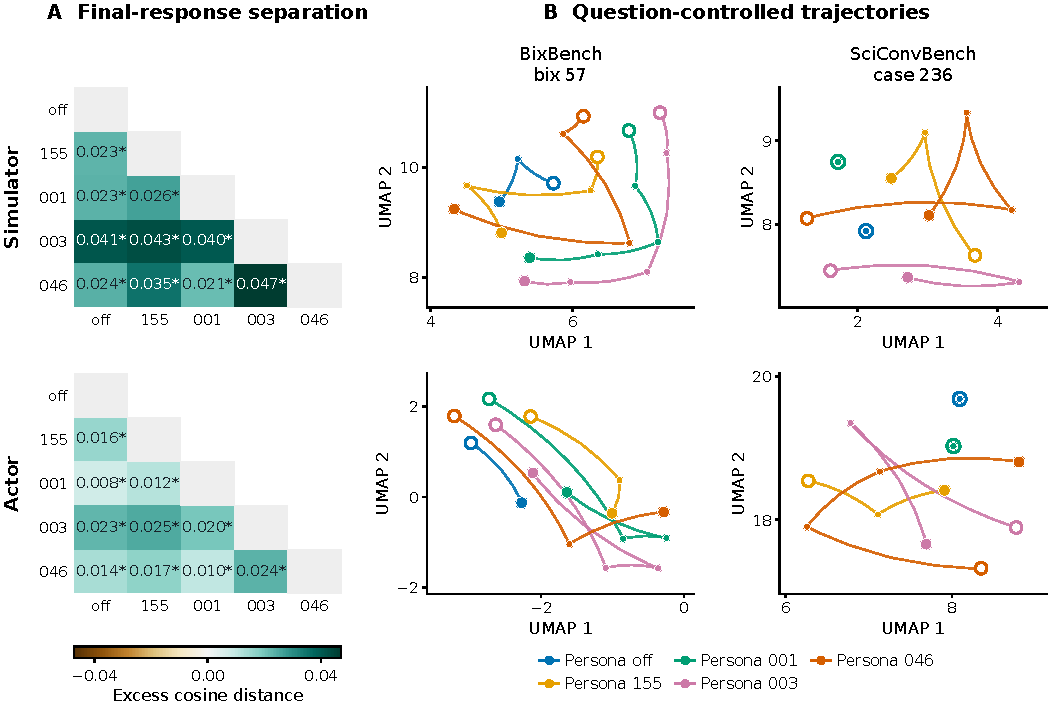
\includegraphics[width=0.75\linewidth]{figures/semantic.pdf}
% Source: Experiment/01_behavioral_diversity/SEMANTIC_FIGURE_CAPTION.md.
\caption{\textbf{Semantic separation and interaction trajectories.}
\textbf{A,} Final-response semantic separation for simulators (top)
and actors (bottom); stars indicate Holm-adjusted $p<0.05$.
\textbf{B,} Example UMAP trajectories for BixBench and SciConvBench.
Hollow circles mark starts, filled circles mark ends, and small dots
mark intermediate messages; overlapping start/end markers denote a single
message.}
\label{fig:semantic-diversity}
\end{figure}

Researcher personas were associated with distinct final responses from both
the simulator and the actor (\figref{fig:semantic-diversity}A).
We compared Qwen3-Embedding-0.6B~\cite{zhang2025qwen3embedding} embeddings within each
domain, measured separation relative to within-persona variation across
questions, and weighted the four domains equally. All
ten persona-pair comparisons showed positive separation in each role
(Holm-adjusted $p<0.05$ in question-wise persona-label permutation
tests~\cite{phipson2010permutation,holm1979sequential}). The effect of personas at the same time extended to the actor's final responses, even though the actor
encountered the researcher profile only through conversation.

Persona diversity appeared in both the intermediate messages and the
overall course of interaction (\figref{fig:semantic-diversity}B).
In BixBench, both simulator and actor trajectories followed distinct paths
with similar overall movement and partial convergence in the
UMAP~\cite{mcinnes2018umap} projection. The shared task thus elicited a
recognizable progression across personas, while the messages produced
along the way remained different. In SciConvBench, the simulator
trajectories differed in their overall patterns, and the corresponding
actor trajectories were distinct as well. These examples illustrate how
diverse researcher behavior was reflected in the agent's responses
throughout the interaction.

Persona-conditioned interactions also drew the actor into more proactive
participation in multi-turn scientific work. The BixBench example involved more interaction iterations
under every persona than under persona off. In SciConvBench, personas 155,
003, and 046 involved three or four interaction iterations, compared with
one iteration for persona off. During these conversations, the actor pursued
specific questions: under persona 046, it successively clarified
the starting structure, magnetic configuration, external pressure, and
convergence criteria. This progression from a brief interaction to targeted
follow-up questions makes the agent an active participant in specifying
how the task should proceed. Such participation is valuable in scientific
collaboration, where initial requests can leave consequential assumptions
and preferences implicit. Continued dialogue gives the researcher and
agent opportunities to make those choices explicit, resolve uncertainty,
and incorporate feedback before committing to an approach.

\subsection{Researcher Profiles Elicit Different Communication Patterns}
\label{sec:behavioral-results}

Profiles that favor detailed communication were accompanied by more
extensive output from both the simulator and the actor
(\figref{fig:pairwise-behavior}A,B). Relative to persona off, personas 155
and 003 elicited an additional 1.12 and 0.61 thousand actor tokens per
episode, respectively. Simulator output also increased under both
profiles; all four comparisons had Holm-adjusted $p<0.05$. These
comparisons matched questions and trials before averaging across
benchmarks. The contrast also appeared between personas: actor output
under 155 and 003 exceeded that under persona 001, whose profile favors
brief, direct communication. Researcher preferences were thus reflected
in how much the agent produced in response, extending the behavioral
variation beyond the simulator itself.

The clearest differences appeared in communication volume. Clarification
recall varied by $-0.28$ to $4.55$ percentage points across persona pairs,
and tool use by $-0.54$ to $0.28$ calls per episode
(\figref{fig:pairwise-behavior}C,D); neither metric showed a pairwise
difference at Holm-adjusted $p<0.05$. These patterns give the benchmark
contrasting communication demands: detailed, accuracy-oriented guidance
under persona 155, concrete explanations under persona 003, and concise
responses under persona 001. Evaluating these settings together makes
responsiveness to researcher preferences an observable part of scientific
collaboration.

% Source: Experiment/01_behavioral_diversity/behavioral_analysis.ipynb,
% figures/compact_behavior/pairwise_behavior_four.pdf; COMPACT_BEHAVIOR.md.
\begin{figure}[!htbp]
    \centering
    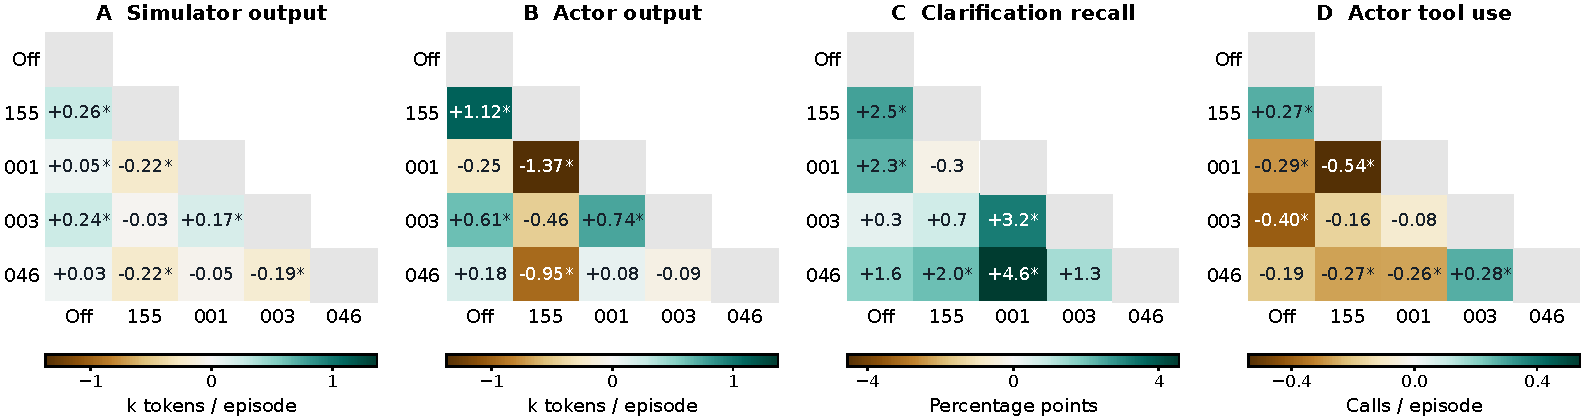
\includegraphics[width=\linewidth]{figures/pairwise_behavior_four.pdf}
    \caption{\textbf{Pairwise behavioral differences.}
Cells show row minus column. \textbf{A, B,} Simulator and actor output
(thousands of tokens per episode). \textbf{C,} SciConvBench clarification
recall (percentage points). \textbf{D,} Actor tool calls per episode.
Stars: \textbf{A, B,} Holm-adjusted $p<0.20$; \textbf{C, D,}
absolute differences above 2 percentage points and 0.2 calls, respectively.}
\label{fig:pairwise-behavior}
\end{figure}


\Needspace{18\baselineskip}
\subsection{Interaction Behavior beyond Final Scores}
\label{sec:interaction-outcomes}

\begin{wrapfigure}{R}{0.58\textwidth}
\vspace{-\intextsep}
\centering
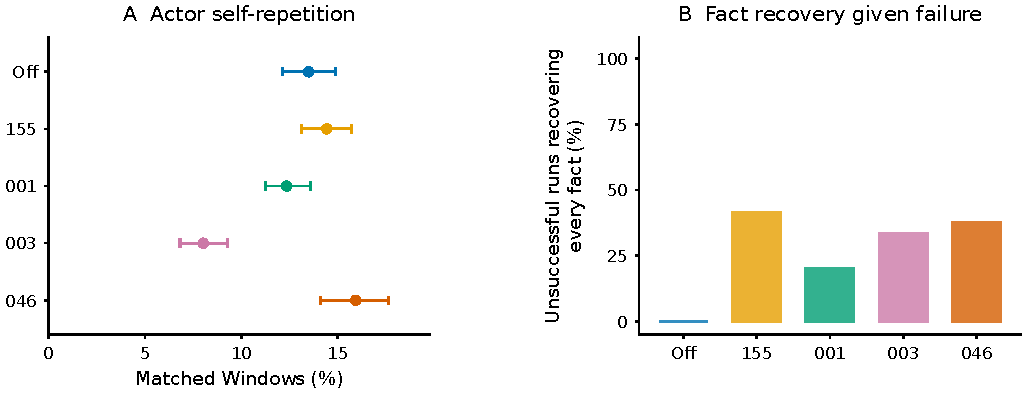
\includegraphics[width=\linewidth]{figures/metric_suite_AB.pdf}
\caption{\textbf{Interaction metrics across researcher personas.}
\textbf{A,} Actor self-repetition; bars show pointwise 95\% study-cluster
confidence intervals. \textbf{B,} Complete-fact recovery among failed
SciConvBench disambiguation episodes.}
\label{fig:metric-suite}
\end{wrapfigure}

The actor returned to its earlier wording to different degrees depending
on the researcher persona (\figref{fig:metric-suite}A). Self-repetition
was 8.03\% under persona 003, compared with 13.50\% for persona off
and 15.94\% under persona 046. These differences are relevant to
conversational mode collapse, where interactions become concentrated in
a few recurring response patterns. CORE evaluates this phenomenon
jointly through mode diversity, lexical repetition, and semantic
stagnation~\cite{pandey2026core}. Extended closed-loop LLM studies
also report semantic collapse, with meanings converging even as surface
wording varies~\cite{kong2026semanticcollapse}. This motivates assessing
self-repetition alongside semantic diversity
(\secref{sec:semantic-results}). In scientific collaboration, avoiding
unnecessary repetition preserves space for targeted clarification,
updated interpretations, and revision of the scientific approach.
The lower self-repetition under persona 003 highlights a setting in
which less of the actor's output reuses its earlier language.
The observed interaction lengths further motivate evaluating multi-turn
scientific work (\figref{fig:interaction-performance}). Every setting received score
contributions from episodes completing after the second iteration. For
persona 003, the cumulative contribution rose from 37.49 at iteration two
to 48.69 at iteration six as later-completing episodes were included.

Information recovery revealed progress during multi-turn scientific work,
including in episodes that ultimately failed (\figref{fig:metric-suite}B).
Within each setting's failed SciConvBench disambiguation episodes,
the case-averaged rate of recovering all required facts ranged from
20.0\% to 41.7\% across the four personas, compared with 0\% for
persona off. The persona-conditioned episodes with complete recovery
contained four to ten interaction iterations, during which the actor
elicited every annotated missing fact before termination. This identifies
a concrete intermediate accomplishment within unsuccessful tasks:
establishing the full factual context needed to formulate a scientific
response. Final scores alone would leave this information-gathering
progress unreported.
